%%%%%%%%%%%%%%%%%%%%%%%%%%%%%%%%%%%%%%%%%
% baposter Portrait Poster
% LaTeX Template
% Version 1.0 (15/5/13)
%
% Created by:
% Brian Amberg (baposter@brian-amberg.de)
%
% This template has been downloaded from:
% http://www.LaTeXTemplates.com
%
% License:
% CC BY-NC-SA 3.0 (http://creativecommons.org/licenses/by-nc-sa/3.0/)
%
%%%%%%%%%%%%%%%%%%%%%%%%%%%%%%%%%%%%%%%%%

%----------------------------------------------------------------------------------------
%	PACKAGES AND OTHER DOCUMENT CONFIGURATIONS
%----------------------------------------------------------------------------------------

\documentclass[a0paper,portrait]{baposter}

\hyphenpenalty=10000
\hbadness=10000

\usepackage[font=small,labelfont=bf]{caption} % Required for specifying captions to tables and figures
\usepackage{booktabs} % Horizontal rules in tables
\usepackage{relsize} % Used for making text smaller in some places

\graphicspath{{figures/}} % Directory in which figures are stored

\definecolor{bordercol}{RGB}{40,40,40} % Border color of content boxes
\definecolor{headercol1}{RGB}{200,215,230} % Background color for the header in the content boxes (left side)
\definecolor{headercol2}{RGB}{220,230,230} % Background color for the header in the content boxes (right side)
\definecolor{headerfontcol}{RGB}{0,0,0} % Text color for the header text in the content boxes
\definecolor{boxcolor}{RGB}{240,250,250} % Background color for the content in the content boxes

\bibliographystyle{unsrt}

\begin{document}

\background{ % Set the background to an image (background.pdf)
% \begin{tikzpicture}[remember picture,overlay]
% \draw (current page.north west)+(-2em,2em) node[anchor=north west]
% {
\includegraphics[height=1.1\textheight]{background}};
% \end{tikzpicture}
}

\begin{poster}{
grid=false,
borderColor=bordercol, % Border color of content boxes
headerColorOne=headercol1, % Background color for the header in the content boxes (left side)
headerColorTwo=headercol2, % Background color for the header in the content boxes (right side)
headerFontColor=headerfontcol, % Text color for the header text in the content boxes
boxColorOne=boxcolor, % Background color for the content in the content boxes
headershape=roundedright, % Specify the rounded corner in the content box headers
headerfont=\Large\sf\bf, % Font modifiers for the text in the content box headers
textborder=rectangle,
background=user,
headerborder=open, % Change to closed for a line under the content box headers
boxshade=plain
}
{}
%
%----------------------------------------------------------------------------------------
%	TITLE AND AUTHOR NAME
%----------------------------------------------------------------------------------------
%
{\sf\bf CLARA: CLAS12 Reconstruction\\and Analysis Framework} % Poster title
{\vspace{1em} Vardan Gyurgyan\hspace{2em}Sebasti\'an Mancilla\hspace{2em}Ricardo Oyarz\'un\\ % Author names
{\smaller gurjyan@jlab.org\hspace{4em}smancill@jlab.org\hspace{4em}oyarzun@jlab.org}} % Author email addresses
{
\includegraphics[scale=0.65]{logo}} % University/lab logo

%----------------------------------------------------------------------------------------
%	INTRODUCTION
%----------------------------------------------------------------------------------------

\headerbox{Introduction}{name=introduction,column=0,row=0}{

The majority of developed physics data processing applications (PDP) are
single, sequential processes that start at a point in time, and advance one
step at a time until they are finished. This approach has noticeable
limitations in the current era of multi-core hardware architectures and
distributed relational data sources.

Contemporary research shows that software programming paradigms and
architectures, such as Service Oriented Architecture (SOA) and Flow Based
Programming (FBP) can withstand future technological pressures and ease
the long term application maintenance.
}

%----------------------------------------------------------------------------------------
%	MATERIALS AND METHODS
%----------------------------------------------------------------------------------------

\headerbox{Component based approach}{name=components,column=0,below=introduction}{

The CLARA framework aims to enhance the efficiency, agility, and productivity
of PDP processes. CLARA is an approach to develop data processing applications
based on the concept of multiple asynchronous processes (software building
blocks), called \textbf{services}, communicating by means of \textbf{data streams}.
Thus, an application is viewed as a system of data streams being transformed
by services.

CLARA is a multilingual framework that supports services in Java,
C++ and Python.
}

%----------------------------------------------------------------------------------------
%	ACKNOWLEDGEMENTS
%----------------------------------------------------------------------------------------

\headerbox{Data dynamic routing}{name=application,column=0,below=components}{

A service composition is comprised of services
that have been assembled to provide the functionality required
to accomplish a specific data processing task.
CLARA makes a clear separation between the service programmer and the data
processing application designer.

Dynamic data routing is stored within the composition field of the transient
metadata.
As a result, CLARA application design can be altered during the application
execution time.
}

%----------------------------------------------------------------------------------------
%	CONCLUSION
%----------------------------------------------------------------------------------------

\headerbox{Conclusion}{name=conclusion,column=0,below=application}{
  Nuclear physics data processing applications written within the CLARA
  framework demonstrated increased performance and simplified maintenance.

  The CLARA application is made of loosely coupled software building blocks.
  CLARA application designer's main focus is the data flow between components.

  This type of application is more fault-tolerant, since faulty blocks can be
  replaced without bringing down the entire application. CLARA application is
  also elastic, since at run-time, new data processing blocks can be added to
  enhance application functionality or existing blocks can be removed to fit
  available computing resources.
}

%----------------------------------------------------------------------------------------
%	REFERENCES
%----------------------------------------------------------------------------------------

\headerbox{References}{name=references,column=0,below=conclusion,above=bottom}{

\smaller % Reduce the font size in this block
\renewcommand{\section}[2]{\vskip 0.05em} % Get rid of the default "References" section title
\nocite{*} % Insert publications even if they are not cited in the poster

\bibliography{biblio} % Use biblio.bib as the bibliography file
}

%----------------------------------------------------------------------------------------
%	RESULTS 1
%----------------------------------------------------------------------------------------

\headerbox{CLAS Application}{name=results,span=2,column=1,row=0}{ % To reduce this block to 1 column width, remove 'span=2'

  The \textbf{CLAS orchestrator} will process a list of input files for
  reconstruction on the JLAB farm nodes. It will wait for DPEs to be started
  on the nodes and it will use them as soon as they are alive.

  For each DPE, the orchestrator will first deploy and link the standard I/O
  services and the user reconstruction services. Then it will configure the
  I/O services to process one of the input files. Finally, it will request to
  start the reconstruction of the file using all cores in the node.

  Each new DPE will be used for I/O and reconstruction (i.e. each node will be
  in charge of reconstructing its own single file). When a DPE finishes a
  file, the orchestrator will use it to process the next file in the list.

%------------------------------------------------

\begin{center}
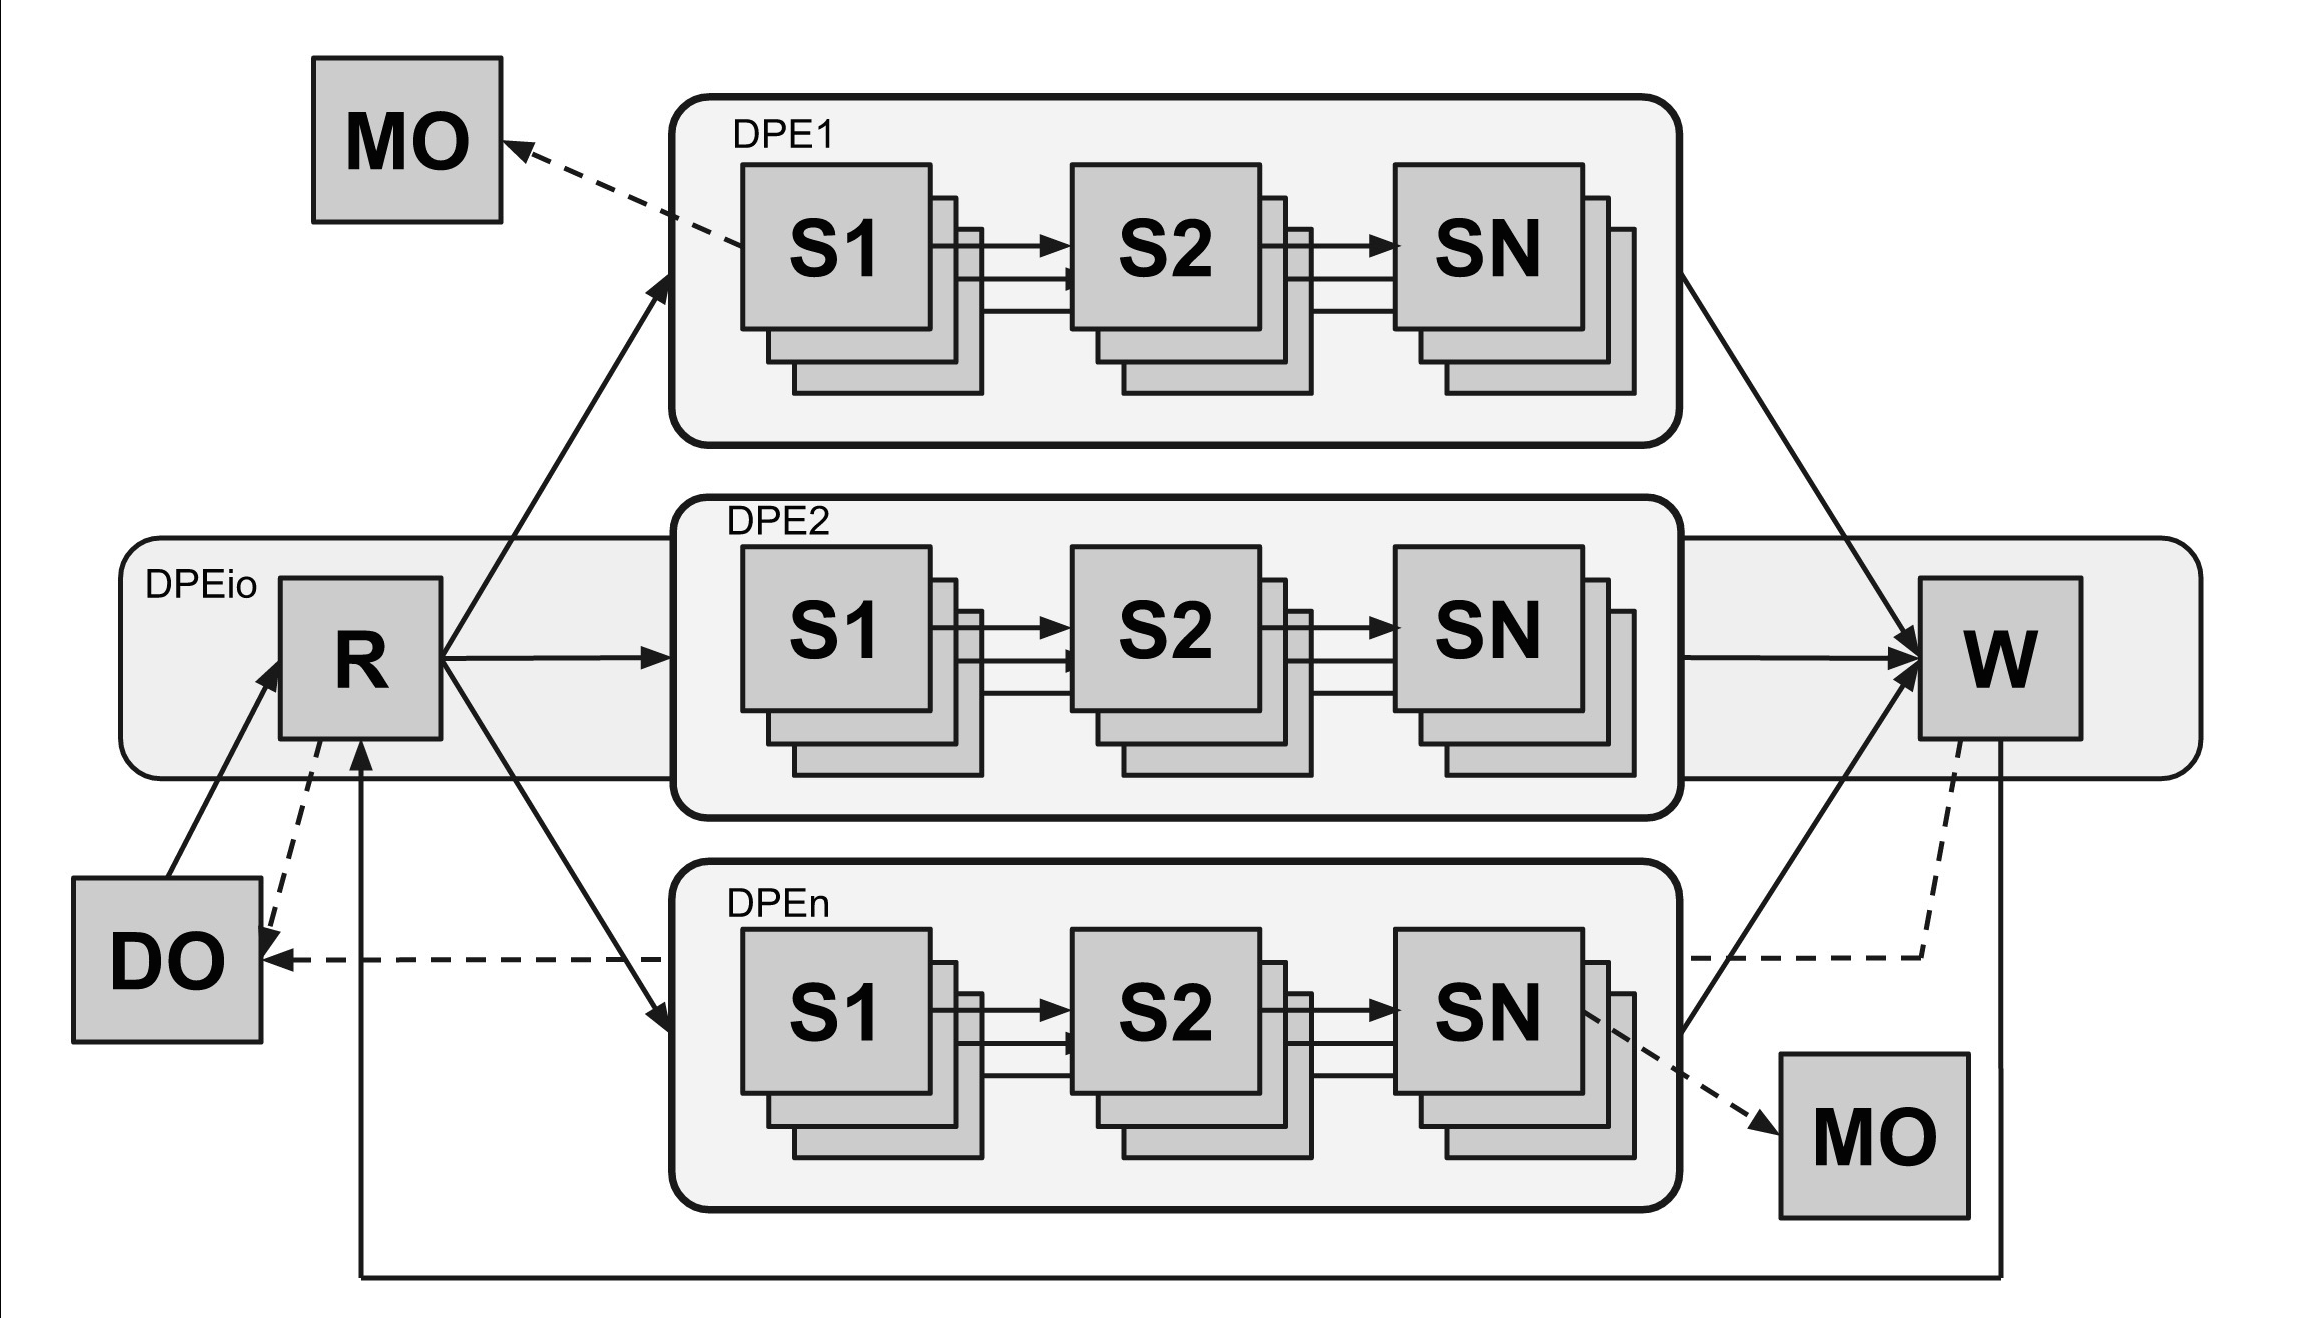
\includegraphics[width=0.7\linewidth]{multinode-reconstruction}
\captionof{figure}{CLAS Reconstruction Application}
\end{center}

The standard reader (R) and writer (W) services and the reconstruction chain
(S1, S2, SN) are deployed on each DPE, all of them linked in a loop. There is
also a data manager (D) service on every node, to handle the staging of the
files. The orchestrator stars and monitors the reconstruction on all available
DPEs.

\begin{center}
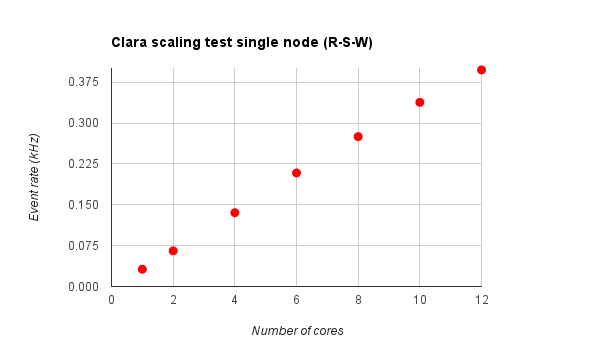
\includegraphics[width=0.49\linewidth]{scaling-singlenode}
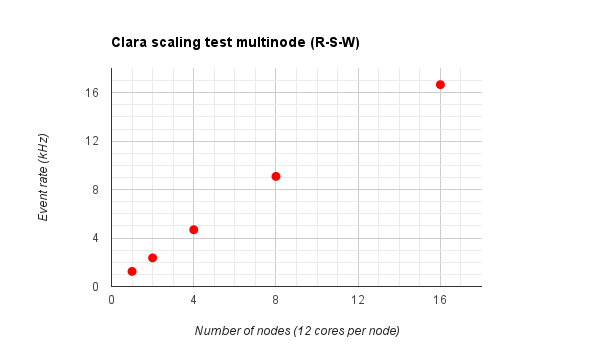
\includegraphics[width=0.49\linewidth]{scaling-multinode}
\captionof{figure}{Clara performance}
\end{center}

As expected, CLARA applications show very good scalability, both on multiple
cores and multiple nodes, allowing maximum occupation of hardware resources.

}

%----------------------------------------------------------------------------------------
%	RESULTS 2
%----------------------------------------------------------------------------------------

\headerbox{REST Interface}{name=webapp,span=2,column=1,below=results,above=bottom}{ % To reduce this block to 1 column width, remove 'span=2'

CLARA includes a REST API, implemented in python. Allowing to query, interact and monitor real time data from the reconstruction process and also allowing to the developer to create his own applications for deployment and monitoring.

\begin{center}
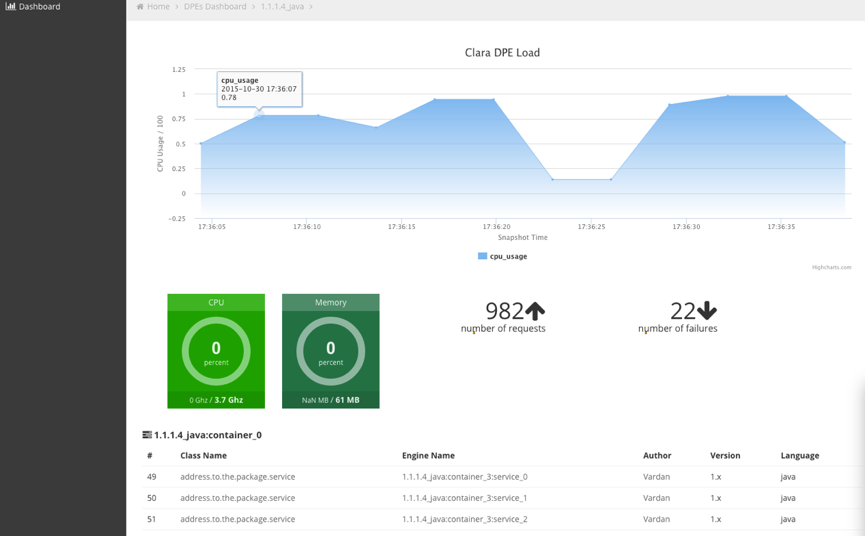
\includegraphics[width=0.45\linewidth]{rest1}
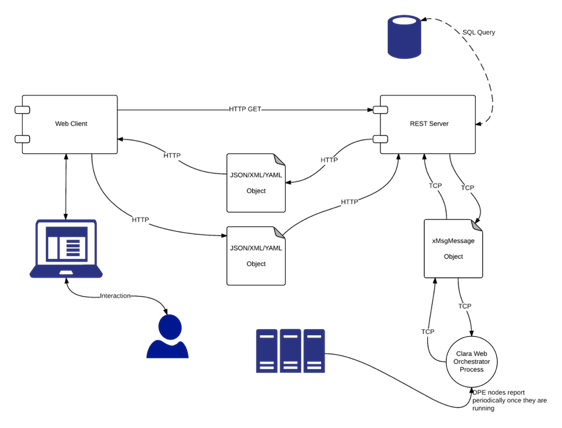
\includegraphics[width=0.45\linewidth]{rest2}
\captionof{figure}{CLAS Reconstruction Web Interface}
\end{center}

}

%----------------------------------------------------------------------------------------

\end{poster}

\end{document}
